\subsection{Assurance Argument}

[SAQIB/ISAAC - 1 pg]

Figure \ref{fig:rta-resolute} represents the assurance argument for run-time assurance architecture. It is divided into three sub-claims. Each sub-claim argues over specific property associated with the system to satisfy the top level claim, i.e., the collision avoidance monitor ensures that a safe flight plan is published. The left most sub-claim argues the correctness of  collision avoidance system architecture that is supported using several sub-claims. These claims are further satisfied using the leaf nodes also known as evidence. In this particular branch of the assurance case we have also demonstrated the ability of Resolute capturing evidence by running external tools (branch labeled with AGREE verification) and pulling the results as part of the assurance argument. Middle sub-claim argues that the collision avoidance system logic is correct. It's achieved using the APT synthesis and reasoning over the stay well clear assessment logic developed by Kestrel. The right most sub-claim guarantees that the backup, i.e., decision from run-time monitor is safe. The evidence for this claim ensures that both the run-time monitor requirements and implementation is correct. 


\begin{figure*}
	\centering
	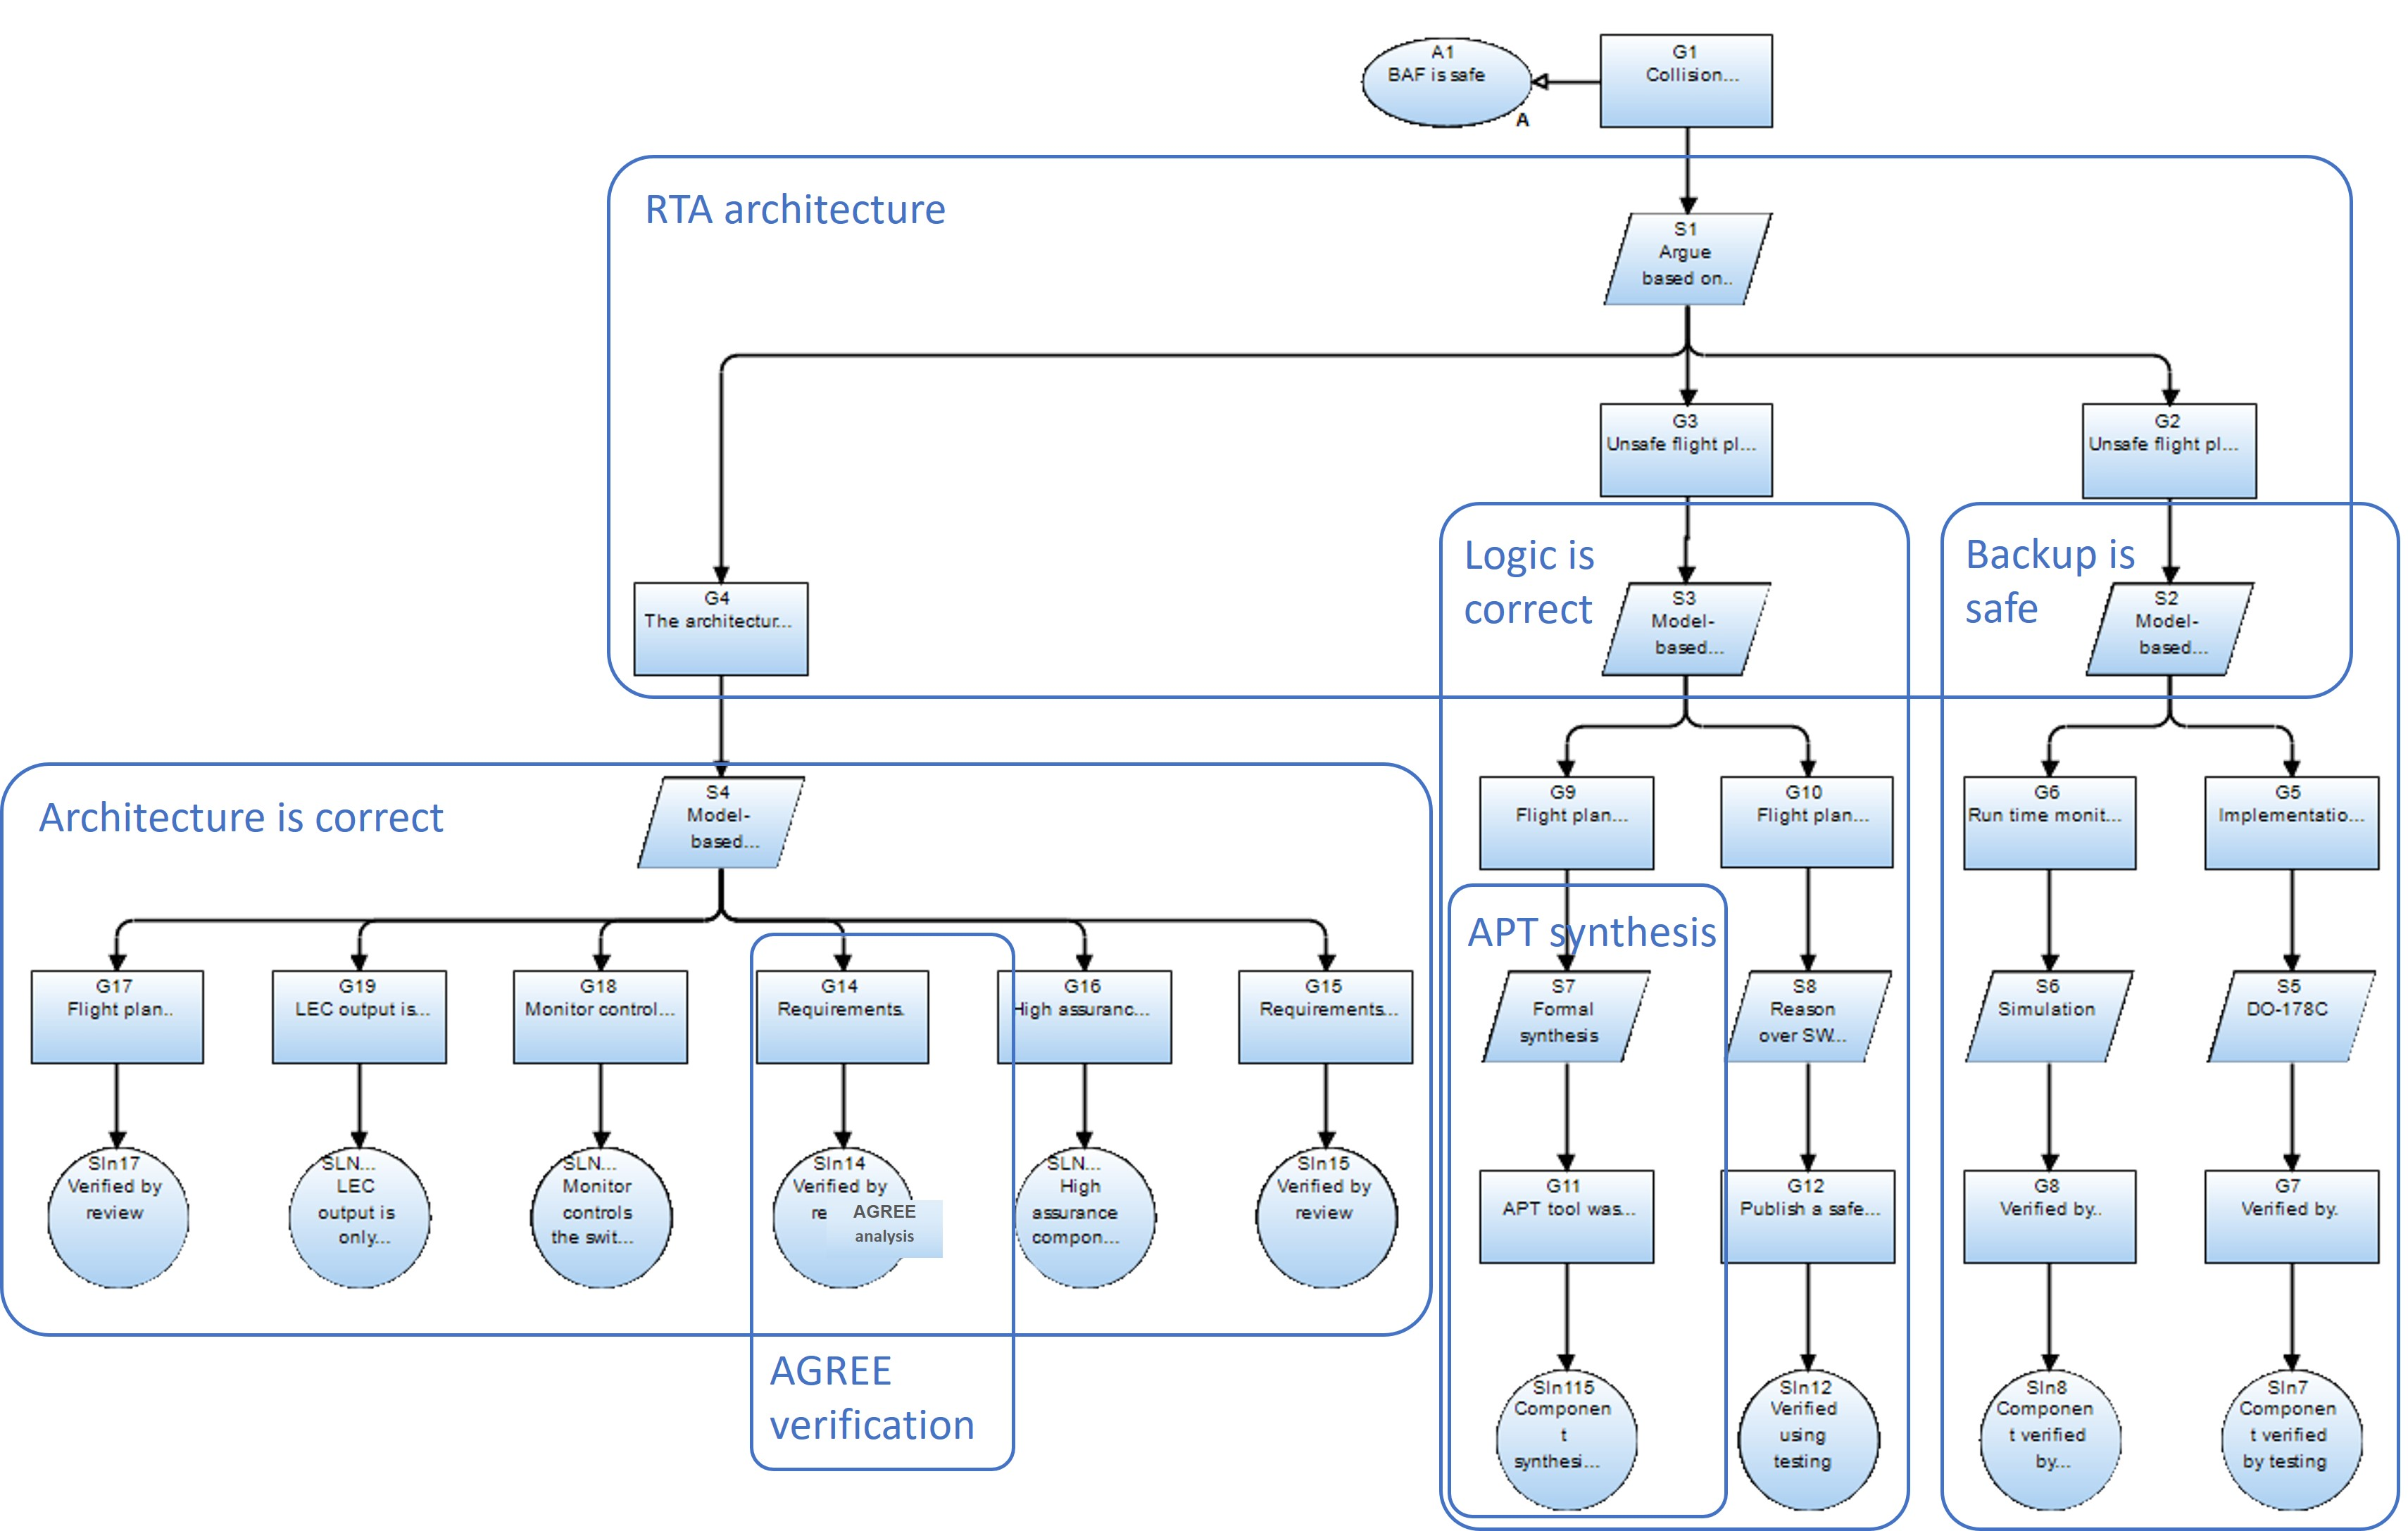
\includegraphics[width=\textwidth]{figures/rta-resolute.jpg}
	\caption{Assurance Argument for run-time assurance generated by Resolute}
	\label{fig:rta-resolute}
\end{figure*}
